% SPDX-License-Identifier: CC-BY-4.0
%
% Copyright (c) 2023 Nelson Vieira
%
% @author Nelson Vieira <nelson0.vieira@gmail.com>
% @license CC-BY-4.0 <https://creativecommons.org/licenses/by/4.0/legalcode.txt>
\chapter*{Appendix}

\section*{Appendix A: Survey}\label{appendix:survey}

\subsection*{Section 1: General knowledge and attitudes towards privacy}

The purpose of this section is to ask general questions about your knowledge
in the area of information privacy.

1. "Privacy is important to me". Do you agree with this statement?

\vspace{0.6cm}
\begin{center}
    \noindent\begin{tabularx}{0.8\textwidth}{ >{\centering\arraybackslash}X >{\centering\arraybackslash}X >{\centering\arraybackslash}X >{\centering\arraybackslash}X >{\centering\arraybackslash}X >{\centering\arraybackslash}X >{\centering\arraybackslash}X >{\centering\arraybackslash}X >{\centering\arraybackslash}X }
        & 1 & 2 & 3 & 4 & 5 & 6 & 7 & \\[0.2cm]
        Disagree & {\huge $\circ$} & {\huge $\circ$} & {\huge $\circ$} & {\huge $\circ$} & {\huge $\circ$} & {\huge $\circ$} & {\huge $\circ$} & Agree
    \end{tabularx}
\end{center}
\vspace{0.6cm}

2. "I know techniques to guarantee privacy and the protection of my data when I use the Internet". Do you agree with this statement?

\vspace{0.6cm}
\begin{center}
    \noindent\begin{tabularx}{0.8\textwidth}{ >{\centering\arraybackslash}X >{\centering\arraybackslash}X >{\centering\arraybackslash}X >{\centering\arraybackslash}X >{\centering\arraybackslash}X >{\centering\arraybackslash}X >{\centering\arraybackslash}X >{\centering\arraybackslash}X >{\centering\arraybackslash}X }
        & 1 & 2 & 3 & 4 & 5 & 6 & 7 & \\[0.2cm]
        Disagree & {\huge $\circ$} & {\huge $\circ$} & {\huge $\circ$} & {\huge $\circ$} & {\huge $\circ$} & {\huge $\circ$} & {\huge $\circ$} & Agree
    \end{tabularx}
\end{center}
\vspace{0.6cm}

3. Could you give examples of techniques or strategies you use to guarantee the privacy and protection of your data?

\vspace{0.6cm}
\begin{center}
    \noindent\begin{tabularx}{0.9\textwidth}{ |>{\raggedright\arraybackslash}X| }
        \hline
        \hspace{0.2cm}Short answer...\vspace{0.5cm} \\
        \hline
    \end{tabularx}
\end{center}
\vspace{0.6cm}

4. Do you think your data privacy is important?

\vspace{0.6cm}
\begin{center}
    \noindent\begin{tabular}{ p{2cm} p{1.3cm} p{1.3cm} p{1.3cm} p{1.3cm} p{1.3cm} p{1.3cm} p{1.3cm} p{2.5cm} }
        & \centering 1 & \centering 2 & \centering 3 & \centering 4 & \centering 5 & \centering 6 & \centering 7 & \\[0.2cm]
        Not at all & \centering {\huge $\circ$} & \centering {\huge $\circ$} & \centering {\huge $\circ$} & \centering {\huge $\circ$} & \centering {\huge $\circ$} & \centering {\huge $\circ$} & \centering {\huge $\circ$} & Very important
    \end{tabular}
\end{center}
\vspace{0.6cm}

5. How do you define data (or digital) privacy?

\vspace{0.6cm}
\begin{center}
    \noindent\begin{tabularx}{0.9\textwidth}{ |>{\raggedright\arraybackslash}X| }
        \hline
        \hspace{0.2cm}Long answer...\vspace{1.75cm} \\
        \hline
    \end{tabularx}
\end{center}
\vspace{0.6cm}

6. Do you think your data privacy is relevant nowadays?

\vspace{0.6cm}
\begin{center}
    \noindent\begin{tabular}{ p{2cm} p{1.3cm} p{1.3cm} p{1.3cm} p{1.3cm} p{1.3cm} p{1.3cm} p{1.3cm} p{2.5cm} }
        & \centering 1 & \centering 2 & \centering 3 & \centering 4 & \centering 5 & \centering 6 & \centering 7 & \\[0.2cm]
        Not at all & \centering {\huge $\circ$} & \centering {\huge $\circ$} & \centering {\huge $\circ$} & \centering {\huge $\circ$} & \centering {\huge $\circ$} & \centering {\huge $\circ$} & \centering {\huge $\circ$} & Very relevant
    \end{tabular}
\end{center}
\vspace{0.6cm}

7. "Data privacy is a human right". Do you agree with this statement?

\vspace{0.6cm}
\begin{center}
    \noindent\begin{tabularx}{0.8\textwidth}{ >{\centering\arraybackslash}X >{\raggedright\arraybackslash}X }
        {\huge $\circ$} & I agree \\[0.2cm]
        {\huge $\circ$} & I disagree \\[0.2cm]
        {\huge $\circ$} & I do not know
    \end{tabularx}
\end{center}
\vspace{0.6cm}

8. "Data privacy is a consumer right". Do you agree with this statement?

\vspace{0.6cm}
\begin{center}
    \noindent\begin{tabularx}{0.8\textwidth}{ >{\centering\arraybackslash}X >{\raggedright\arraybackslash}X }
        {\huge $\circ$} & I agree \\[0.2cm]
        {\huge $\circ$} & I disagree \\[0.2cm]
        {\huge $\circ$} & I do not know
    \end{tabularx}
\end{center}
\vspace{0.6cm}

9. In your opinion, are security and privacy synonymous?

\vspace{0.6cm}
\begin{center}
    \noindent\begin{tabularx}{0.8\textwidth}{ >{\centering\arraybackslash}X >{\raggedright\arraybackslash}X }
        {\huge $\circ$} & Yes \\[0.2cm]
        {\huge $\circ$} & No
    \end{tabularx}
\end{center}
\vspace{0.6cm}

10. How familiar are you with the following terms?

\vspace{0.6cm}
\begin{center}
    \noindent\begin{tabular}{ p{4.5cm} p{3cm} p{4cm} p{3cm} }
        & I Know well & I have some knowledge & I do not know \\[0.4cm]
        Cookie & {\huge $\circ$} & {\huge $\circ$} & {\huge $\circ$} \\[0.2cm]
        Wireless networks & {\huge $\circ$} & {\huge $\circ$} & {\huge $\circ$} \\[0.2cm]
        Wi-Fi & {\huge $\circ$} & {\huge $\circ$} & {\huge $\circ$} \\[0.2cm]
        Internet of Things & {\huge $\circ$} & {\huge $\circ$} & {\huge $\circ$} \\[0.2cm]
        Data protection & {\huge $\circ$} & {\huge $\circ$} & {\huge $\circ$} \\[0.2cm]
        Ad hoc network (wireless) & {\huge $\circ$} & {\huge $\circ$} & {\huge $\circ$} \\[0.2cm]
        Ubiquitous computing & {\huge $\circ$} & {\huge $\circ$} & {\huge $\circ$} \\[0.2cm]
        Privacy assistant & {\huge $\circ$} & {\huge $\circ$} & {\huge $\circ$} \\[0.2cm]
        Blockchain & {\huge $\circ$} & {\huge $\circ$} & {\huge $\circ$} \\[0.2cm]
        Differential privacy & {\huge $\circ$} & {\huge $\circ$} & {\huge $\circ$}
    \end{tabular}
\end{center}
\vspace{0.6cm}

11. Do you think your data is stored/collected when you use the internet?

\vspace{0.6cm}
\begin{center}
    \noindent\begin{tabularx}{0.8\textwidth}{ >{\centering\arraybackslash}X >{\raggedright\arraybackslash}X }
        {\huge $\circ$} & Yes \\[0.2cm]
        {\huge $\circ$} & No \\[0.2cm]
        {\huge $\circ$} & I do not know
    \end{tabularx}
\end{center}
\vspace{0.6cm}

12. What means do you think are used to collect your data?

\vspace{0.6cm}
\begin{center}
    \begin{tabular}{r *{4}{ p{6cm} }}
        {\Large $\square$}\hspace{1cm} & Sound (microphones, recorders, etc.) \\[0.2cm]
        {\Large $\square$}\hspace{1cm} & Image (webcams, scanners, etc.) \\[0.2cm]
        {\Large $\square$}\hspace{1cm} & Online Surveys / Questionnaires \\[0.2cm]
        {\Large $\square$}\hspace{1cm} & Hackers (illegal means) \\[0.2cm]
        {\Large $\square$}\hspace{1cm} & Cookies \\[0.2cm]
        {\Large $\square$}\hspace{1cm} & None \\[0.2cm]
        \hhline{~|-|>{\arrayrulecolor{black}}-|>{\arrayrulecolor{black}}-|}
        {\Large $\square$}\hspace{1cm} & \multicolumn{1}{!{\color{black}\vline}c!{\color{black}\vline}}{Another option...} \\ \cline{2-3}
    \end{tabular}
\end{center}
\vspace{0.6cm}

13. What kind of information can be extracted using the collected data?

\vspace{0.6cm}
\begin{center}
    \begin{tabular}{r *{4}{ p{6cm} }}
        {\Large $\square$}\hspace{1cm} & Visited websites information \\[0.2cm]
        {\Large $\square$}\hspace{1cm} & Work productivity \\[0.2cm]
        {\Large $\square$}\hspace{1cm} & Georeferencing data \\[0.2cm]
        {\Large $\square$}\hspace{1cm} & Online habits \\[0.2cm]
        {\Large $\square$}\hspace{1cm} & Online shoppping \\[0.2cm]
        \hhline{~|-|>{\arrayrulecolor{black}}-|>{\arrayrulecolor{black}}-|}
        {\Large $\square$}\hspace{1cm} & \multicolumn{1}{!{\color{black}\vline}c!{\color{black}\vline}}{Another option...} \\ \cline{2-3}
    \end{tabular}
\end{center}
\vspace{0.6cm}

14. For what purposes can organizations use your data?

\vspace{0.6cm}
\begin{center}
    \begin{tabular}{r *{4}{ p{6cm} }}
        {\Large $\square$}\hspace{1cm} & Improve internet usage \\[0.2cm]
        {\Large $\square$}\hspace{1cm} & Costumer profile \\[0.2cm]
        {\Large $\square$}\hspace{1cm} & Targeted advertising \\[0.2cm]
        {\Large $\square$}\hspace{1cm} & Advertising adapted to the nearest locations \\[0.2cm]
        {\Large $\square$}\hspace{1cm} & Selling data to third parties \\[0.2cm]
        \hhline{~|-|>{\arrayrulecolor{black}}-|>{\arrayrulecolor{black}}-|}
        {\Large $\square$}\hspace{1cm} & \multicolumn{1}{!{\color{black}\vline}c!{\color{black}\vline}}{Another option...} \\ \cline{2-3}
    \end{tabular}
\end{center}
\vspace{0.6cm}

15. Which organizations do you consider to have the best privacy behaviour?

\vspace{0.6cm}
\begin{center}
    \begin{tabular}{r *{4}{ p{6cm} }}
        {\Large $\square$}\hspace{1cm} & Amazon \\[0.2cm]
        {\Large $\square$}\hspace{1cm} & Apple \\[0.2cm]
        {\Large $\square$}\hspace{1cm} & Google \\[0.2cm]
        {\Large $\square$}\hspace{1cm} & Meta (Facebook, Whatsapp, Instagram) \\[0.2cm]
        {\Large $\square$}\hspace{1cm} & Microsoft \\[0.2cm]
        {\Large $\square$}\hspace{1cm} & Samsung \\[0.2cm]
        {\Large $\square$}\hspace{1cm} & IBM \\[0.2cm]
        {\Large $\square$}\hspace{1cm} & ScienceSoft \\[0.2cm]
        {\Large $\square$}\hspace{1cm} & PTC \\[0.2cm]
        {\Large $\square$}\hspace{1cm} & Cisco \\[0.2cm]
        {\Large $\square$}\hspace{1cm} & Huawei \\[0.2cm]
        {\Large $\square$}\hspace{1cm} & GE Digital \\[0.2cm]
        {\Large $\square$}\hspace{1cm} & Bosch \\[0.2cm]
        {\Large $\square$}\hspace{1cm} & Siemens \\[0.2cm]
        \hhline{~|-|>{\arrayrulecolor{black}}-|>{\arrayrulecolor{black}}-|}
        {\Large $\square$}\hspace{1cm} & \multicolumn{1}{!{\color{black}\vline}c!{\color{black}\vline}}{Other...} \\ \cline{2-3}
    \end{tabular}
\end{center}
\vspace{0.6cm}

16. Which organizations do you consider to have the worst privacy behaviour?

\vspace{0.6cm}
\begin{center}
    \begin{tabular}{r *{4}{ p{6cm} }}
        {\Large $\square$}\hspace{1cm} & Amazon \\[0.2cm]
        {\Large $\square$}\hspace{1cm} & Apple \\[0.2cm]
        {\Large $\square$}\hspace{1cm} & Google \\[0.2cm]
        {\Large $\square$}\hspace{1cm} & Meta (Facebook, Whatsapp, Instagram) \\[0.2cm]
        {\Large $\square$}\hspace{1cm} & Microsoft \\[0.2cm]
        {\Large $\square$}\hspace{1cm} & Samsung \\[0.2cm]
        {\Large $\square$}\hspace{1cm} & IBM \\[0.2cm]
        {\Large $\square$}\hspace{1cm} & ScienceSoft \\[0.2cm]
        {\Large $\square$}\hspace{1cm} & PTC \\[0.2cm]
        {\Large $\square$}\hspace{1cm} & Cisco \\[0.2cm]
        {\Large $\square$}\hspace{1cm} & Huawei \\[0.2cm]
        {\Large $\square$}\hspace{1cm} & GE Digital \\[0.2cm]
        {\Large $\square$}\hspace{1cm} & Bosch \\[0.2cm]
        {\Large $\square$}\hspace{1cm} & Siemens \\[0.2cm]
        \hhline{~|-|>{\arrayrulecolor{black}}-|>{\arrayrulecolor{black}}-|}
        {\Large $\square$}\hspace{1cm} & \multicolumn{1}{!{\color{black}\vline}c!{\color{black}\vline}}{Other...} \\ \cline{2-3}
    \end{tabular}
\end{center}
\vspace{0.6cm}

17. During your day-to-day life, how often do you use your phone to access the internet?

\vspace{0.6cm}
\begin{center}
    \noindent\begin{tabular}{ p{2cm} p{1.3cm} p{1.3cm} p{1.3cm} p{1.3cm} p{1.3cm} p{1.3cm} p{1.3cm} p{2.5cm} }
        & \centering 1 & \centering 2 & \centering 3 & \centering 4 & \centering 5 & \centering 6 & \centering 7 & \\[0.2cm]
        Never & \centering {\huge $\circ$} & \centering {\huge $\circ$} & \centering {\huge $\circ$} & \centering {\huge $\circ$} & \centering {\huge $\circ$} & \centering {\huge $\circ$} & \centering {\huge $\circ$} & Very often
    \end{tabular}
\end{center}
\vspace{0.6cm}

18. "I am concerned about my privacy when using my mobile phone when accessing the internet". Do you agree with this statement?

\vspace{0.6cm}
\begin{center}
    \noindent\begin{tabularx}{0.8\textwidth}{ >{\centering\arraybackslash}X >{\centering\arraybackslash}X >{\centering\arraybackslash}X >{\centering\arraybackslash}X >{\centering\arraybackslash}X >{\centering\arraybackslash}X >{\centering\arraybackslash}X >{\centering\arraybackslash}X >{\centering\arraybackslash}X }
        & 1 & 2 & 3 & 4 & 5 & 6 & 7 & \\[0.2cm]
        Disagree & {\huge $\circ$} & {\huge $\circ$} & {\huge $\circ$} & {\huge $\circ$} & {\huge $\circ$} & {\huge $\circ$} & {\huge $\circ$} & Agree
    \end{tabularx}
\end{center}
\vspace{0.6cm}

19. "I consider that accessing the internet through my phone is safer than through a computer". Do you agree with this statement?

\vspace{0.6cm}
\begin{center}
    \noindent\begin{tabularx}{0.8\textwidth}{ >{\centering\arraybackslash}X >{\centering\arraybackslash}X >{\centering\arraybackslash}X >{\centering\arraybackslash}X >{\centering\arraybackslash}X >{\centering\arraybackslash}X >{\centering\arraybackslash}X >{\centering\arraybackslash}X >{\centering\arraybackslash}X }
        & 1 & 2 & 3 & 4 & 5 & 6 & 7 & \\[0.2cm]
        Disagree & {\huge $\circ$} & {\huge $\circ$} & {\huge $\circ$} & {\huge $\circ$} & {\huge $\circ$} & {\huge $\circ$} & {\huge $\circ$} & Agree
    \end{tabularx}
\end{center}
\vspace{0.6cm}

20. "I try to block the collection of data from applications installed on my phone". Do you agree with this statement?

\vspace{0.6cm}
\begin{center}
    \noindent\begin{tabularx}{0.8\textwidth}{ >{\centering\arraybackslash}X >{\centering\arraybackslash}X >{\centering\arraybackslash}X >{\centering\arraybackslash}X >{\centering\arraybackslash}X >{\centering\arraybackslash}X >{\centering\arraybackslash}X >{\centering\arraybackslash}X >{\centering\arraybackslash}X }
        & 1 & 2 & 3 & 4 & 5 & 6 & 7 & \\[0.2cm]
        Disagree & {\huge $\circ$} & {\huge $\circ$} & {\huge $\circ$} & {\huge $\circ$} & {\huge $\circ$} & {\huge $\circ$} & {\huge $\circ$} & Agree
    \end{tabularx}
\end{center}
\vspace{0.6cm}

21. When using a website, do you usually read the Privacy Policy?

\vspace{0.6cm}
\begin{center}
    \noindent\begin{tabularx}{0.8\textwidth}{ >{\centering\arraybackslash}X >{\raggedright\arraybackslash}X }
        {\huge $\circ$} & Yes, always \\[0.2cm]
        {\huge $\circ$} & Yes, almost always \\[0.2cm]
        {\huge $\circ$} & No, because I am not interested \\[0.2cm]
        {\huge $\circ$} & No, but I know what it means or what happens
    \end{tabularx}
\end{center}
\vspace{0.6cm}

22. How often do you allow the use of cookies?

\vspace{0.6cm}
\begin{center}
    \noindent\begin{tabularx}{0.8\textwidth}{ >{\centering\arraybackslash}X >{\centering\arraybackslash}X >{\centering\arraybackslash}X >{\centering\arraybackslash}X >{\centering\arraybackslash}X >{\centering\arraybackslash}X >{\centering\arraybackslash}X >{\centering\arraybackslash}X >{\centering\arraybackslash}X }
        & 1 & 2 & 3 & 4 & 5 & 6 & 7 & \\[0.2cm]
        Never & {\huge $\circ$} & {\huge $\circ$} & {\huge $\circ$} & {\huge $\circ$} & {\huge $\circ$} & {\huge $\circ$} & {\huge $\circ$} & Always
    \end{tabularx}
\end{center}
\vspace{0.6cm}

23. When you accept / become aware of the cookies policy, why do you take this decision?

\vspace{0.6cm}
\begin{center}
    \noindent\begin{tabular}{r *{4}{ p{6cm} }}
        {\huge $\circ$}\hspace{1cm} & It is the only way to access the website \\[0.2cm]
        {\huge $\circ$}\hspace{1cm} & I understand what it is about and I agree with the policy presented \\[0.2cm]
        {\huge $\circ$}\hspace{1cm} & I don't understand what this is about but it doesn't seem relevant to me \\[0.2cm]
        \hhline{~|-|>{\arrayrulecolor{black}}-|>{\arrayrulecolor{black}}-|}
        {\huge $\circ$}\hspace{1cm} & \multicolumn{1}{!{\color{black}\vline}c!{\color{black}\vline}}{Other...} \\ \cline{2-3}
    \end{tabular}
\end{center}
\vspace{0.6cm}

24. Are you aware of the concept of "profiling" or "automated processing of personal information"?

\vspace{0.6cm}
\begin{center}
    \noindent\begin{tabularx}{0.8\textwidth}{ >{\centering\arraybackslash}X >{\raggedright\arraybackslash}X }
        {\huge $\circ$} & Yes \\[0.2cm]
        {\huge $\circ$} & No
    \end{tabularx}
\end{center}
\vspace{0.6cm}

25. Do you consider that your internet activity contributes to the development of profiling?

\vspace{0.6cm}
\begin{center}
    \noindent\begin{tabularx}{0.8\textwidth}{ >{\centering\arraybackslash}X >{\raggedright\arraybackslash}X }
        {\huge $\circ$} & Yes \\[0.2cm]
        {\huge $\circ$} & No \\[0.2cm]
        {\huge $\circ$} & I do not know
    \end{tabularx}
\end{center}
\vspace{0.6cm}

26. Are you aware of regulations such as the General Data Protection Regulation or the California Consumer Privacy Act?

\vspace{0.6cm}
\begin{center}
    \noindent\begin{tabularx}{0.8\textwidth}{ >{\centering\arraybackslash}X >{\raggedright\arraybackslash}X }
        {\huge $\circ$} & Yes, I fully understand the regulations \\[0.2cm]
        {\huge $\circ$} & Yes, but it's not absolutely clear to me what it represents \\[0.2cm]
        {\huge $\circ$} & No
    \end{tabularx}
\end{center}
\vspace{0.6cm}

27. If you answered yes, how did you learn about the 'General Data Protection Regulation' or the 'California Consumer Privacy Act'?

\vspace{0.6cm}
\begin{center}
    \begin{tabular}{r *{4}{ p{6cm} }}
        {\Large $\square$}\hspace{1cm} & Internet \\[0.2cm]
        {\Large $\square$}\hspace{1cm} & Television \\[0.2cm]
        {\Large $\square$}\hspace{1cm} & Newspapers \\[0.2cm]
        {\Large $\square$}\hspace{1cm} & Friends \\[0.2cm]
        {\Large $\square$}\hspace{1cm} & Work \\[0.2cm]
        \hhline{~|-|>{\arrayrulecolor{black}}-|>{\arrayrulecolor{black}}-|}
        {\Large $\square$}\hspace{1cm} & \multicolumn{1}{!{\color{black}\vline}c!{\color{black}\vline}}{Other...} \\ \cline{2-3}
    \end{tabular}
\end{center}
\vspace{0.6cm}

28. Are you interested in finding out more about regulations or legislation related to digital privacy?

\vspace{0.6cm}
\begin{center}
    \noindent\begin{tabular}{ p{2cm} p{1.3cm} p{1.3cm} p{1.3cm} p{1.3cm} p{1.3cm} p{1.3cm} p{1.3cm} p{2.5cm} }
        & \centering 1 & \centering 2 & \centering 3 & \centering 4 & \centering 5 & \centering 6 & \centering 7 & \\[0.2cm]
        Not at all & \centering {\huge $\circ$} & \centering {\huge $\circ$} & \centering {\huge $\circ$} & \centering {\huge $\circ$} & \centering {\huge $\circ$} & \centering {\huge $\circ$} & \centering {\huge $\circ$} & Very much
    \end{tabular}
\end{center}
\vspace{0.6cm}

29. According to the General Data Protection Regulation, personal data is:

\vspace{0.6cm}
\begin{center}
    \noindent\begin{tabularx}{0.8\textwidth}{ >{\centering\arraybackslash}X >{\raggedright\arraybackslash}X }
        {\huge $\circ$} & Just name, email, date of birth and tax identification number \\[0.2cm]
        {\huge $\circ$} & All of the above and bank details \\[0.2cm]
        {\huge $\circ$} & All of the above and medical information \\[0.2cm]
        {\huge $\circ$} & Any information relating to an identified or identifiable natural person
    \end{tabularx}
\end{center}
\vspace{0.6cm}

30. "My data was more protected after the implementation of regulations such as the General Data Protection Regulation". Do you agree with this statement?

\vspace{0.6cm}
\begin{center}
    \noindent\begin{tabularx}{0.8\textwidth}{ >{\centering\arraybackslash}X >{\centering\arraybackslash}X >{\centering\arraybackslash}X >{\centering\arraybackslash}X >{\centering\arraybackslash}X >{\centering\arraybackslash}X >{\centering\arraybackslash}X >{\centering\arraybackslash}X >{\centering\arraybackslash}X }
        & 1 & 2 & 3 & 4 & 5 & 6 & 7 & \\[0.2cm]
        Disagree & {\huge $\circ$} & {\huge $\circ$} & {\huge $\circ$} & {\huge $\circ$} & {\huge $\circ$} & {\huge $\circ$} & {\huge $\circ$} & Agree
    \end{tabularx}
\end{center}
\vspace{0.6cm}

\subsection*{Section 2: Disposition for sharing personal information}

This section is intended to ask questions to generally understand your willingness to share personal information.

1. What kind of personal information are you willing to share at any time?

\vspace{0.6cm}
\begin{center}
    \begin{tabular}{r *{4}{ p{6cm} }}
        {\Large $\square$}\hspace{1cm} & Age \\[0.2cm]
        {\Large $\square$}\hspace{1cm} & Complete name \\[0.2cm]
        {\Large $\square$}\hspace{1cm} & Date of birth \\[0.2cm]
        {\Large $\square$}\hspace{1cm} & Genre \\[0.2cm]
        {\Large $\square$}\hspace{1cm} & Religion \\[0.2cm]
        {\Large $\square$}\hspace{1cm} & Complete name of parents \\[0.2cm]
        {\Large $\square$}\hspace{1cm} & Marital status \\[0.2cm]
        {\Large $\square$}\hspace{1cm} & Home address \\[0.2cm]
        {\Large $\square$}\hspace{1cm} & Work address \\[0.2cm]
        {\Large $\square$}\hspace{1cm} & Nationality \\[0.2cm]
        {\Large $\square$}\hspace{1cm} & Qualifications \\[0.2cm]
        {\Large $\square$}\hspace{1cm} & Professional experience \\[0.2cm]
        {\Large $\square$}\hspace{1cm} & Height \\[0.2cm]
        {\Large $\square$}\hspace{1cm} & Weight \\[0.2cm]
        {\Large $\square$}\hspace{1cm} & Phone/mobile number \\[0.2cm]
        {\Large $\square$}\hspace{1cm} & Region of birth \\[0.2cm]
        {\Large $\square$}\hspace{1cm} & Ethnic group \\[0.2cm]
        {\Large $\square$}\hspace{1cm} & Signature \\[0.2cm]
        {\Large $\square$}\hspace{1cm} & Spouse's name \\[0.2cm]
        {\Large $\square$}\hspace{1cm} & Email \\[0.2cm]
        {\Large $\square$}\hspace{1cm} & Health condition \\[0.2cm]
        {\Large $\square$}\hspace{1cm} & Face photo \\[0.2cm]
        {\Large $\square$}\hspace{1cm} & Full body photography \\[0.2cm]
        {\Large $\square$}\hspace{1cm} & Username \\[0.2cm]
        {\Large $\square$}\hspace{1cm} & Copy of citizen card \\[0.2cm]
        {\Large $\square$}\hspace{1cm} & Fingerprint \\[0.2cm]
        {\Large $\square$}\hspace{1cm} & Licenses
    \end{tabular}
\end{center}
\vspace{0.6cm}

2. In what situations are you willing to provide more personal information?

\vspace{0.6cm}
\begin{center}
    \begin{tabular}{r *{4}{ p{6cm} }}
        {\Large $\square$}\hspace{1cm} & Renew your citizen card \\[0.2cm]
        {\Large $\square$}\hspace{1cm} & Medical consultation (face to face) \\[0.2cm]
        {\Large $\square$}\hspace{1cm} & Take out health insurance \\[0.2cm]
        {\Large $\square$}\hspace{1cm} & Create new bank account \\[0.2cm]
        {\Large $\square$}\hspace{1cm} & For contact tracing \\[0.2cm]
        {\Large $\square$}\hspace{1cm} & Confined in the hospital \\[0.2cm]
        {\Large $\square$}\hspace{1cm} & Make a new Internet/Mobile plan \\[0.2cm]
        {\Large $\square$}\hspace{1cm} & Online shopping \\[0.2cm]
        {\Large $\square$}\hspace{1cm} & Apply for a bank loan or credit card \\[0.2cm]
        {\Large $\square$}\hspace{1cm} & Online medical consultation \\[0.2cm]
        {\Large $\square$}\hspace{1cm} & Request loyalty/discount cards \\[0.2cm]
        {\Large $\square$}\hspace{1cm} & None
    \end{tabular}
\end{center}
\vspace{0.6cm}

3. Do you agree to share health data that can identify you with health professionals?

\vspace{0.6cm}
\begin{center}
    \noindent\begin{tabularx}{0.8\textwidth}{ >{\centering\arraybackslash}X >{\raggedright\arraybackslash}X }
        {\huge $\circ$} & Yes, I agree \\[0.2cm]
        {\huge $\circ$} & Maybe if asked first \\[0.2cm]
        {\huge $\circ$} & No, I disagree \\[0.2cm]
        {\huge $\circ$} & I do not know
    \end{tabularx}
\end{center}
\vspace{0.6cm}

4. Do you agree to share health data that cannot identify you with health professionals?

\vspace{0.6cm}
\begin{center}
    \noindent\begin{tabularx}{0.8\textwidth}{ >{\centering\arraybackslash}X >{\raggedright\arraybackslash}X }
        {\huge $\circ$} & Yes, I agree \\[0.2cm]
        {\huge $\circ$} & Maybe if asked first \\[0.2cm]
        {\huge $\circ$} & No, I disagree \\[0.2cm]
        {\huge $\circ$} & I do not know
    \end{tabularx}
\end{center}
\vspace{0.6cm}

5. What kind of applications do you have installed on your smartphone?

\vspace{0.6cm}
\begin{center}
    \begin{tabular}{r *{4}{ p{6cm} }}
        {\Large $\square$}\hspace{1cm} & Social media \\[0.2cm]
        {\Large $\square$}\hspace{1cm} & Instant messages \\[0.2cm]
        {\Large $\square$}\hspace{1cm} & Email \\[0.2cm]
        {\Large $\square$}\hspace{1cm} & Browser \\[0.2cm]
        {\Large $\square$}\hspace{1cm} & Navigation (ex. GPS) \\[0.2cm]
        {\Large $\square$}\hspace{1cm} & Anti-virus \\[0.2cm]
        {\Large $\square$}\hspace{1cm} & Online shopping \\[0.2cm]
        {\Large $\square$}\hspace{1cm} & Digital Wallet \\[0.2cm]
        {\Large $\square$}\hspace{1cm} & Photo/video editing \\[0.2cm]
        {\Large $\square$}\hspace{1cm} & Contact tracing \\[0.2cm]
        {\Large $\square$}\hspace{1cm} & Online banking \\[0.2cm]
        \hhline{~|-|>{\arrayrulecolor{black}}-|>{\arrayrulecolor{black}}-|}
        {\Large $\square$}\hspace{1cm} & \multicolumn{1}{!{\color{black}\vline}c!{\color{black}\vline}}{Other...} \\ \cline{2-3}
    \end{tabular}
\end{center}
\vspace{0.6cm}

6. Before sharing your data, do you consult any of the following information?

\vspace{0.6cm}
\begin{center}
    \begin{tabular}{r *{4}{ p{6cm} }}
        {\Large $\square$}\hspace{1cm} & Privacy policy \\[0.2cm]
        {\Large $\square$}\hspace{1cm} & Terms and conditions \\[0.2cm]
        {\Large $\square$}\hspace{1cm} & Purpose of data collection \\[0.2cm]
        {\Large $\square$}\hspace{1cm} & Consent Form \\[0.2cm]
        {\Large $\square$}\hspace{1cm} & Privacy notice \\[0.2cm]
        {\Large $\square$}\hspace{1cm} & Reliability of the organization/institution \\[0.2cm]
        {\Large $\square$}\hspace{1cm} & I do not consult any information
    \end{tabular}
\end{center}
\vspace{0.6cm}

7. How often do you find privacy policies?

\vspace{0.6cm}
\begin{center}
    \noindent\begin{tabularx}{0.8\textwidth}{ >{\centering\arraybackslash}X >{\raggedright\arraybackslash}X }
        {\huge $\circ$} & Almost everyday \\[0.2cm]
        {\huge $\circ$} & Once a week \\[0.2cm]
        {\huge $\circ$} & Once a month \\[0.2cm]
        {\huge $\circ$} & Very rarely \\[0.2cm]
        {\huge $\circ$} & Never
    \end{tabularx}
\end{center}
\vspace{0.6cm}

8. Are you aware of the duties of a Data Protection Officer (DPO)?

\vspace{0.6cm}
\begin{center}
    \noindent\begin{tabularx}{0.8\textwidth}{ >{\centering\arraybackslash}X >{\raggedright\arraybackslash}X }
        {\huge $\circ$} & Yes \\[0.2cm]
        {\huge $\circ$} & No
    \end{tabularx}
\end{center}
\vspace{0.6cm}

9. "I am interested in knowing where and how my personal information is used." Do you agree with this statement?

\vspace{0.6cm}
\begin{center}
    \noindent\begin{tabularx}{0.8\textwidth}{ >{\centering\arraybackslash}X >{\raggedright\arraybackslash}X }
        {\huge $\circ$} & I agree \\[0.2cm]
        {\huge $\circ$} & I do not agree nor disagree \\[0.2cm]
        {\huge $\circ$} & I disagree
    \end{tabularx}
\end{center}
\vspace{0.6cm}

10. "I am not familiar with the purpose of data collection but would like to know more". Do you agree with this statement?

\vspace{0.6cm}
\begin{center}
    \noindent\begin{tabularx}{0.8\textwidth}{ >{\centering\arraybackslash}X >{\raggedright\arraybackslash}X }
        {\huge $\circ$} & I agree \\[0.2cm]
        {\huge $\circ$} & I do not agree nor disagree \\[0.2cm]
        {\huge $\circ$} & I disagree
    \end{tabularx}
\end{center}
\vspace{0.6cm}

11. "The length (or number of words) of the privacy notice affects my willingness to read it." Do you agree with this statement?

\vspace{0.6cm}
\begin{center}
    \noindent\begin{tabularx}{0.8\textwidth}{ >{\centering\arraybackslash}X >{\raggedright\arraybackslash}X }
        {\huge $\circ$} & I agree \\[0.2cm]
        {\huge $\circ$} & I do not agree nor disagree \\[0.2cm]
        {\huge $\circ$} & I disagree
    \end{tabularx}
\end{center}
\vspace{0.6cm}

12. "The font size of the privacy notice affects my willingness to read it." Do you agree with this statement?

\vspace{0.6cm}
\begin{center}
    \noindent\begin{tabularx}{0.8\textwidth}{ >{\centering\arraybackslash}X >{\raggedright\arraybackslash}X }
        {\huge $\circ$} & I agree \\[0.2cm]
        {\huge $\circ$} & I do not agree nor disagree \\[0.2cm]
        {\huge $\circ$} & I disagree
    \end{tabularx}
\end{center}
\vspace{0.6cm}

13. "Usually, I'm afraid I won't be able to use a product or service if I don't agree with the privacy notice." Do you agree with this statement?

\vspace{0.6cm}
\begin{center}
    \noindent\begin{tabularx}{0.8\textwidth}{ >{\centering\arraybackslash}X >{\raggedright\arraybackslash}X }
        {\huge $\circ$} & I agree \\[0.2cm]
        {\huge $\circ$} & I do not agree nor disagree \\[0.2cm]
        {\huge $\circ$} & I disagree
    \end{tabularx}
\end{center}
\vspace{0.6cm}

14. "I don't need to read the privacy notice if I trust the institution". Do you agree with this statement?

\vspace{0.6cm}
\begin{center}
    \noindent\begin{tabularx}{0.8\textwidth}{ >{\centering\arraybackslash}X >{\raggedright\arraybackslash}X }
        {\huge $\circ$} & I agree \\[0.2cm]
        {\huge $\circ$} & I do not agree nor disagree \\[0.2cm]
        {\huge $\circ$} & I disagree
    \end{tabularx}
\end{center}
\vspace{0.6cm}

\subsection*{Section 3: Privacy concerns}

This section aims to ask questions related to possible fears associated with sharing personal information.

1. How concerned are you about organizations collecting and using your online activity?

\vspace{0.6cm}
\begin{center}
    \noindent\begin{tabular}{ p{2cm} p{1.3cm} p{1.3cm} p{1.3cm} p{1.3cm} p{1.3cm} p{1.3cm} p{1.3cm} p{2.5cm} }
        & \centering 1 & \centering 2 & \centering 3 & \centering 4 & \centering 5 & \centering 6 & \centering 7 & \\[0.2cm]
        Not at all & \centering {\huge $\circ$} & \centering {\huge $\circ$} & \centering {\huge $\circ$} & \centering {\huge $\circ$} & \centering {\huge $\circ$} & \centering {\huge $\circ$} & \centering {\huge $\circ$} & Very concerned
    \end{tabular}
\end{center}
\vspace{0.6cm}

2. How concerned are you about organizations sharing your data with third parties?

\vspace{0.6cm}
\begin{center}
    \noindent\begin{tabular}{ p{2cm} p{1.3cm} p{1.3cm} p{1.3cm} p{1.3cm} p{1.3cm} p{1.3cm} p{1.3cm} p{2.5cm} }
        & \centering 1 & \centering 2 & \centering 3 & \centering 4 & \centering 5 & \centering 6 & \centering 7 & \\[0.2cm]
        Not at all & \centering {\huge $\circ$} & \centering {\huge $\circ$} & \centering {\huge $\circ$} & \centering {\huge $\circ$} & \centering {\huge $\circ$} & \centering {\huge $\circ$} & \centering {\huge $\circ$} & Very concerned
    \end{tabular}
\end{center}
\vspace{0.6cm}

3. How concerned are you about organizations tracking your online behavior and thus obtaining your personal data?

\vspace{0.6cm}
\begin{center}
    \noindent\begin{tabular}{ p{2cm} p{1.3cm} p{1.3cm} p{1.3cm} p{1.3cm} p{1.3cm} p{1.3cm} p{1.3cm} p{2.5cm} }
        & \centering 1 & \centering 2 & \centering 3 & \centering 4 & \centering 5 & \centering 6 & \centering 7 & \\[0.2cm]
        Not at all & \centering {\huge $\circ$} & \centering {\huge $\circ$} & \centering {\huge $\circ$} & \centering {\huge $\circ$} & \centering {\huge $\circ$} & \centering {\huge $\circ$} & \centering {\huge $\circ$} & Very concerned
    \end{tabular}
\end{center}
\vspace{0.6cm}

4. How concerned are you about public institutions or intelligence services analyzing your online movements?

\vspace{0.6cm}
\begin{center}
    \noindent\begin{tabular}{ p{2cm} p{1.3cm} p{1.3cm} p{1.3cm} p{1.3cm} p{1.3cm} p{1.3cm} p{1.3cm} p{2.5cm} }
        & \centering 1 & \centering 2 & \centering 3 & \centering 4 & \centering 5 & \centering 6 & \centering 7 & \\[0.2cm]
        Not at all & \centering {\huge $\circ$} & \centering {\huge $\circ$} & \centering {\huge $\circ$} & \centering {\huge $\circ$} & \centering {\huge $\circ$} & \centering {\huge $\circ$} & \centering {\huge $\circ$} & Very concerned
    \end{tabular}
\end{center}
\vspace{0.6cm}

5. How concerned are you that other people obtain your personal data without your consent?

\vspace{0.6cm}
\begin{center}
    \noindent\begin{tabular}{ p{2cm} p{1.3cm} p{1.3cm} p{1.3cm} p{1.3cm} p{1.3cm} p{1.3cm} p{1.3cm} p{2.5cm} }
        & \centering 1 & \centering 2 & \centering 3 & \centering 4 & \centering 5 & \centering 6 & \centering 7 & \\[0.2cm]
        Not at all & \centering {\huge $\circ$} & \centering {\huge $\circ$} & \centering {\huge $\circ$} & \centering {\huge $\circ$} & \centering {\huge $\circ$} & \centering {\huge $\circ$} & \centering {\huge $\circ$} & Very concerned
    \end{tabular}
\end{center}
\vspace{0.6cm}

6. How concerned are you that other people find information about you online?

\vspace{0.6cm}
\begin{center}
    \noindent\begin{tabular}{ p{2cm} p{1.3cm} p{1.3cm} p{1.3cm} p{1.3cm} p{1.3cm} p{1.3cm} p{1.3cm} p{2.5cm} }
        & \centering 1 & \centering 2 & \centering 3 & \centering 4 & \centering 5 & \centering 6 & \centering 7 & \\[0.2cm]
        Not at all & \centering {\huge $\circ$} & \centering {\huge $\circ$} & \centering {\huge $\circ$} & \centering {\huge $\circ$} & \centering {\huge $\circ$} & \centering {\huge $\circ$} & \centering {\huge $\circ$} & Very concerned
    \end{tabular}
\end{center}
\vspace{0.6cm}

7. How concerned are you that other people are disclosing information about you without your knowledge?

\vspace{0.6cm}
\begin{center}
    \noindent\begin{tabular}{ p{2cm} p{1.3cm} p{1.3cm} p{1.3cm} p{1.3cm} p{1.3cm} p{1.3cm} p{1.3cm} p{2.5cm} }
        & \centering 1 & \centering 2 & \centering 3 & \centering 4 & \centering 5 & \centering 6 & \centering 7 & \\[0.2cm]
        Not at all & \centering {\huge $\circ$} & \centering {\huge $\circ$} & \centering {\huge $\circ$} & \centering {\huge $\circ$} & \centering {\huge $\circ$} & \centering {\huge $\circ$} & \centering {\huge $\circ$} & Very concerned
    \end{tabular}
\end{center}
\vspace{0.6cm}

8. How concerned are you about other people sharing your personal data (photos, address, mobile phone number, etc.) with others without your consent?

\vspace{0.6cm}
\begin{center}
    \noindent\begin{tabular}{ p{2cm} p{1.3cm} p{1.3cm} p{1.3cm} p{1.3cm} p{1.3cm} p{1.3cm} p{1.3cm} p{2.5cm} }
        & \centering 1 & \centering 2 & \centering 3 & \centering 4 & \centering 5 & \centering 6 & \centering 7 & \\[0.2cm]
        Not at all & \centering {\huge $\circ$} & \centering {\huge $\circ$} & \centering {\huge $\circ$} & \centering {\huge $\circ$} & \centering {\huge $\circ$} & \centering {\huge $\circ$} & \centering {\huge $\circ$} & Very concerned
    \end{tabular}
\end{center}
\vspace{0.6cm}

9. How concerned are you that other people publish your personal data (photos, address, mobile phone number, etc.) on the internet without your consent?

\vspace{0.6cm}
\begin{center}
    \noindent\begin{tabular}{ p{2cm} p{1.3cm} p{1.3cm} p{1.3cm} p{1.3cm} p{1.3cm} p{1.3cm} p{1.3cm} p{2.5cm} }
        & \centering 1 & \centering 2 & \centering 3 & \centering 4 & \centering 5 & \centering 6 & \centering 7 & \\[0.2cm]
        Not at all & \centering {\huge $\circ$} & \centering {\huge $\circ$} & \centering {\huge $\circ$} & \centering {\huge $\circ$} & \centering {\huge $\circ$} & \centering {\huge $\circ$} & \centering {\huge $\circ$} & Very concerned
    \end{tabular}
\end{center}
\vspace{0.6cm}

10. How concerned are you about an unknown person claiming to be you on the internet?

\vspace{0.6cm}
\begin{center}
    \noindent\begin{tabular}{ p{2cm} p{1.3cm} p{1.3cm} p{1.3cm} p{1.3cm} p{1.3cm} p{1.3cm} p{1.3cm} p{2.5cm} }
        & \centering 1 & \centering 2 & \centering 3 & \centering 4 & \centering 5 & \centering 6 & \centering 7 & \\[0.2cm]
        Not at all & \centering {\huge $\circ$} & \centering {\huge $\circ$} & \centering {\huge $\circ$} & \centering {\huge $\circ$} & \centering {\huge $\circ$} & \centering {\huge $\circ$} & \centering {\huge $\circ$} & Very concerned
    \end{tabular}
\end{center}
\vspace{0.6cm}

11. How concerned are you about the possibility that someone may misuse your identity on the internet?

\vspace{0.6cm}
\begin{center}
    \noindent\begin{tabular}{ p{2cm} p{1.3cm} p{1.3cm} p{1.3cm} p{1.3cm} p{1.3cm} p{1.3cm} p{1.3cm} p{2.5cm} }
        & \centering 1 & \centering 2 & \centering 3 & \centering 4 & \centering 5 & \centering 6 & \centering 7 & \\[0.2cm]
        Not at all & \centering {\huge $\circ$} & \centering {\huge $\circ$} & \centering {\huge $\circ$} & \centering {\huge $\circ$} & \centering {\huge $\circ$} & \centering {\huge $\circ$} & \centering {\huge $\circ$} & Very concerned
    \end{tabular}
\end{center}
\vspace{0.6cm}

\subsection*{Section 4: Current online habits and practices}

This section brings together general questions about using the Internet in your daily life.

1. Do you have internet access at home?

\vspace{0.6cm}
\begin{center}
    \begin{tabular}{r *{4}{ p{6cm} }}
        {\Large $\square$}\hspace{1cm} & By Wi-fi or Ethernet cable \\[0.2cm]
        {\Large $\square$}\hspace{1cm} & By mobile network (eg. 4G or 5G) \\[0.2cm]
        {\Large $\square$}\hspace{1cm} & No
    \end{tabular}
\end{center}
\vspace{0.6cm}

2. How often do you use the internet?

\vspace{0.6cm}
\begin{center}
    \noindent\begin{tabularx}{0.8\textwidth}{ >{\centering\arraybackslash}X >{\raggedright\arraybackslash}X }
        {\huge $\circ$} & Everyday \\[0.2cm]
        {\huge $\circ$} & 2 or 3 days a week \\[0.2cm]
        {\huge $\circ$} & Once a week \\[0.2cm]
        {\huge $\circ$} & Once a month \\[0.2cm]
        {\huge $\circ$} & Never
    \end{tabularx}
\end{center}
\vspace{0.6cm}

3. How much time do you spend per day surfing the internet?

\vspace{0.6cm}
\begin{center}
    \noindent\begin{tabularx}{0.8\textwidth}{ >{\centering\arraybackslash}X >{\raggedright\arraybackslash}X }
        {\huge $\circ$} & <1 hour \\[0.2cm]
        {\huge $\circ$} & 1-2 hours \\[0.2cm]
        {\huge $\circ$} & 2-5 hours \\[0.2cm]
        {\huge $\circ$} & 5-10 hours \\[0.2cm]
        {\huge $\circ$} & 10+ hours
    \end{tabularx}
\end{center}
\vspace{0.6cm}

4. What device(s) do you use to access the internet?

\vspace{0.6cm}
\begin{center}
    \begin{tabular}{r *{4}{ p{6cm} }}
        {\Large $\square$}\hspace{1cm} & Computer \\[0.2cm]
        {\Large $\square$}\hspace{1cm} & Laptop \\[0.2cm]
        {\Large $\square$}\hspace{1cm} & Tablet \\[0.2cm]
        {\Large $\square$}\hspace{1cm} & Phone \\[0.2cm]
        \hhline{~|-|>{\arrayrulecolor{black}}-|>{\arrayrulecolor{black}}-|}
        {\Large $\square$}\hspace{1cm} & \multicolumn{1}{!{\color{black}\vline}c!{\color{black}\vline}}{Other...} \\ \cline{2-3}
    \end{tabular}
\end{center}
\vspace{0.6cm}

5. For what purposes do you use the internet?

\vspace{0.6cm}
\begin{center}
    \begin{tabular}{r *{4}{ p{6cm} }}
        {\Large $\square$}\hspace{1cm} & Search for information about politics, health, etc. \\[0.2cm]
        {\Large $\square$}\hspace{1cm} & Social media \\[0.2cm]
        {\Large $\square$}\hspace{1cm} & Online shopping \\[0.2cm]
        {\Large $\square$}\hspace{1cm} & Consult email \\[0.2cm]
        {\Large $\square$}\hspace{1cm} & Listen to music \\[0.2cm]
        {\Large $\square$}\hspace{1cm} & Play videogames \\[0.2cm]
        {\Large $\square$}\hspace{1cm} & Watch movies/series \\[0.2cm]
        {\Large $\square$}\hspace{1cm} & Study online \\[0.2cm]
        {\Large $\square$}\hspace{1cm} & Look for a job \\[0.2cm]
        {\Large $\square$}\hspace{1cm} & Work \\[0.2cm]
        {\Large $\square$}\hspace{1cm} & Publish to a blog or online journal \\[0.2cm]
        \hhline{~|-|>{\arrayrulecolor{black}}-|>{\arrayrulecolor{black}}-|}
        {\Large $\square$}\hspace{1cm} & \multicolumn{1}{!{\color{black}\vline}c!{\color{black}\vline}}{Other...} \\ \cline{2-3}
    \end{tabular}
\end{center}
\vspace{0.6cm}

6. What platforms/applications do you use in your day-to-day life?

\vspace{0.6cm}
\begin{center}
    \begin{tabular}{r *{4}{ p{6cm} }}
        {\Large $\square$}\hspace{1cm} & Social media \\[0.2cm]
        {\Large $\square$}\hspace{1cm} & Instant messages \\[0.2cm]
        {\Large $\square$}\hspace{1cm} & Email \\[0.2cm]
        {\Large $\square$}\hspace{1cm} & Browser \\[0.2cm]
        {\Large $\square$}\hspace{1cm} & Online shopping \\[0.2cm]
        {\Large $\square$}\hspace{1cm} & Photo/video editing \\[0.2cm]
        {\Large $\square$}\hspace{1cm} & Online banking \\[0.2cm]
        {\Large $\square$}\hspace{1cm} & Anti-virus \\[0.2cm]
        {\Large $\square$}\hspace{1cm} & Contact tracing \\[0.2cm]
        {\Large $\square$}\hspace{1cm} & Delivery services
    \end{tabular}
\end{center}
\vspace{0.6cm}

7. On social media, do you usually:

\vspace{0.6cm}
\begin{center}
    \begin{tabular}{r *{4}{ p{6cm} }}
        {\Large $\square$}\hspace{1cm} & Use your own photo showing your face as your profile picture \\[0.2cm]
        {\Large $\square$}\hspace{1cm} & Use your real and full name \\[0.2cm]
        {\Large $\square$}\hspace{1cm} & Put the date of birth, age and other information \\[0.2cm]
        {\Large $\square$}\hspace{1cm} & Do not post information that could identify me
    \end{tabular}
\end{center}
\vspace{0.6cm}

8. Your activity on social media goes through:

\vspace{0.6cm}
\begin{center}
    \begin{tabular}{r *{4}{ p{6cm} }}
        {\Large $\square$}\hspace{1cm} & Sharing photos of children/family members who are minors \\[0.2cm]
        {\Large $\square$}\hspace{1cm} & Follow any elected officials, candidates for office or other political figures \\[0.2cm]
        {\Large $\square$}\hspace{1cm} & Follow celebrities, or people with some notoriety \\[0.2cm]
        {\Large $\square$}\hspace{1cm} & Post links to/from business, sport or articles \\[0.2cm]
        {\Large $\square$}\hspace{1cm} & Post links to political stories or other articles \\[0.2cm]
        {\Large $\square$}\hspace{1cm} & Post political or social opinions \\[0.2cm]
        {\Large $\square$}\hspace{1cm} & I don't use social media
    \end{tabular}
\end{center}
\vspace{0.6cm}

\subsection*{Section 5: Profile identification}

This section brings together more specific questions about using profiles to make it easier to create personalized experiences.

1. Do you know the concept of profiling?

\vspace{0.6cm}
\begin{center}
    \noindent\begin{tabularx}{0.9\textwidth}{ |>{\raggedright\arraybackslash}X| }
        \hline
        \hspace{0.2cm}Long answer...\vspace{1.75cm} \\
        \hline
    \end{tabularx}
\end{center}
\vspace{0.6cm}

2. If a law enforcement officer asks for your personal data, are you willing to share it?

\vspace{0.6cm}
\begin{center}
    \noindent\begin{tabularx}{0.8\textwidth}{ >{\centering\arraybackslash}X >{\raggedright\arraybackslash}X }
        {\huge $\circ$} & Yes \\[0.2cm]
        {\huge $\circ$} & No \\[0.2cm]
        {\huge $\circ$} & I do not know
    \end{tabularx}
\end{center}
\vspace{0.6cm}

3. In what situations are you willing to provide personal data when data collection is disclosed?

\vspace{0.6cm}
\begin{center}
    \begin{tabular}{r *{4}{ p{6cm} }}
        {\Large $\square$}\hspace{1cm} & Renew your citizen card \\[0.2cm]
        {\Large $\square$}\hspace{1cm} & Medical consultation (face to face) \\[0.2cm]
        {\Large $\square$}\hspace{1cm} & Take out health insurance \\[0.2cm]
        {\Large $\square$}\hspace{1cm} & Create new bank account \\[0.2cm]
        {\Large $\square$}\hspace{1cm} & For contact tracing \\[0.2cm]
        {\Large $\square$}\hspace{1cm} & Confined in the hospital \\[0.2cm]
        {\Large $\square$}\hspace{1cm} & Make a new Internet/Mobile plan \\[0.2cm]
        {\Large $\square$}\hspace{1cm} & Online shopping \\[0.2cm]
        {\Large $\square$}\hspace{1cm} & Apply for a bank loan or credit card \\[0.2cm]
        {\Large $\square$}\hspace{1cm} & Online medical consultation \\[0.2cm]
        {\Large $\square$}\hspace{1cm} & Request loyalty/discount cards \\[0.2cm]
        {\Large $\square$}\hspace{1cm} & None
    \end{tabular}
\end{center}
\vspace{0.6cm}

4. In what situations are you willing to provide personal data when data collection is not disclosed?

\vspace{0.6cm}
\begin{center}
    \begin{tabular}{r *{4}{ p{6cm} }}
        {\Large $\square$}\hspace{1cm} & Renew your citizen card \\[0.2cm]
        {\Large $\square$}\hspace{1cm} & Medical consultation (face to face) \\[0.2cm]
        {\Large $\square$}\hspace{1cm} & Take out health insurance \\[0.2cm]
        {\Large $\square$}\hspace{1cm} & Create new bank account \\[0.2cm]
        {\Large $\square$}\hspace{1cm} & For contact tracing \\[0.2cm]
        {\Large $\square$}\hspace{1cm} & Confined in the hospital \\[0.2cm]
        {\Large $\square$}\hspace{1cm} & Make a new Internet/Mobile plan \\[0.2cm]
        {\Large $\square$}\hspace{1cm} & Online shopping \\[0.2cm]
        {\Large $\square$}\hspace{1cm} & Apply for a bank loan or credit card \\[0.2cm]
        {\Large $\square$}\hspace{1cm} & Online medical consultation \\[0.2cm]
        {\Large $\square$}\hspace{1cm} & Request loyalty/discount cards \\[0.2cm]
        {\Large $\square$}\hspace{1cm} & None
    \end{tabular}
\end{center}
\vspace{0.6cm}

5. Do you usually answer online questionnaires when they are requested?

\vspace{0.6cm}
\begin{center}
    \noindent\begin{tabularx}{0.8\textwidth}{ >{\centering\arraybackslash}X >{\centering\arraybackslash}X >{\centering\arraybackslash}X >{\centering\arraybackslash}X >{\centering\arraybackslash}X >{\centering\arraybackslash}X >{\centering\arraybackslash}X >{\centering\arraybackslash}X >{\centering\arraybackslash}X }
        & 1 & 2 & 3 & 4 & 5 & 6 & 7 & \\[0.2cm]
        Never & {\huge $\circ$} & {\huge $\circ$} & {\huge $\circ$} & {\huge $\circ$} & {\huge $\circ$} & {\huge $\circ$} & {\huge $\circ$} & Always
    \end{tabularx}
\end{center}
\vspace{0.6cm}

6. When answering questionnaires, do you enter any false/incorrect information?

\vspace{0.6cm}
\begin{center}
    \noindent\begin{tabularx}{0.8\textwidth}{ >{\centering\arraybackslash}X >{\centering\arraybackslash}X >{\centering\arraybackslash}X >{\centering\arraybackslash}X >{\centering\arraybackslash}X >{\centering\arraybackslash}X >{\centering\arraybackslash}X >{\centering\arraybackslash}X >{\centering\arraybackslash}X }
        & 1 & 2 & 3 & 4 & 5 & 6 & 7 & \\[0.2cm]
        Never & {\huge $\circ$} & {\huge $\circ$} & {\huge $\circ$} & {\huge $\circ$} & {\huge $\circ$} & {\huge $\circ$} & {\huge $\circ$} & Always
    \end{tabularx}
\end{center}
\vspace{0.6cm}

7. When creating an account on an online platform, have you ever entered false personal data?

\vspace{0.6cm}
\begin{center}
    \noindent\begin{tabularx}{0.8\textwidth}{ >{\centering\arraybackslash}X >{\centering\arraybackslash}X >{\centering\arraybackslash}X >{\centering\arraybackslash}X >{\centering\arraybackslash}X >{\centering\arraybackslash}X >{\centering\arraybackslash}X >{\centering\arraybackslash}X >{\centering\arraybackslash}X }
        & 1 & 2 & 3 & 4 & 5 & 6 & 7 & \\[0.2cm]
        Never & {\huge $\circ$} & {\huge $\circ$} & {\huge $\circ$} & {\huge $\circ$} & {\huge $\circ$} & {\huge $\circ$} & {\huge $\circ$} & Always
    \end{tabularx}
\end{center}
\vspace{0.6cm}

7.1. If yes, why did you enter this false data?

\vspace{0.6cm}
\begin{center}
    \begin{tabular}{r *{4}{ p{6cm} }}
        {\Large $\square$}\hspace{1cm} & I am creating a temporary account \\[0.2cm]
        {\Large $\square$}\hspace{1cm} & I do not want to disclose any kind of personal data, I want maximum privacy \\[0.2cm]
        {\Large $\square$}\hspace{1cm} & I do not find this type of data(s) relevant \\[0.2cm]
        {\Large $\square$}\hspace{1cm} & I want to access the content of the platform as soon as possible \\[0.2cm]
        {\Large $\square$}\hspace{1cm} & I entered the data by mistake \\[0.2cm]
        {\Large $\square$}\hspace{1cm} & I don't have a specific reason \\[0.2cm]
        {\Large $\square$}\hspace{1cm} & The number of data to be inserted is too large \\[0.2cm]
        \hhline{~|-|>{\arrayrulecolor{black}}-|>{\arrayrulecolor{black}}-|}
        {\Large $\square$}\hspace{1cm} & \multicolumn{1}{!{\color{black}\vline}c!{\color{black}\vline}}{Other...} \\ \cline{2-3}
    \end{tabular}
\end{center}
\vspace{0.6cm}

7.2. When you have to enter false data, what types of false data do you enter?

\vspace{0.6cm}
\begin{center}
    \begin{tabular}{r *{4}{ p{6cm} }}
        {\Large $\square$}\hspace{1cm} & Age \\[0.2cm]
        {\Large $\square$}\hspace{1cm} & Complete name \\[0.2cm]
        {\Large $\square$}\hspace{1cm} & Date of birth \\[0.2cm]
        {\Large $\square$}\hspace{1cm} & Genre \\[0.2cm]
        {\Large $\square$}\hspace{1cm} & Religion \\[0.2cm]
        {\Large $\square$}\hspace{1cm} & Complete name of parents \\[0.2cm]
        {\Large $\square$}\hspace{1cm} & Marital status \\[0.2cm]
        {\Large $\square$}\hspace{1cm} & Home address \\[0.2cm]
        {\Large $\square$}\hspace{1cm} & Work address \\[0.2cm]
        {\Large $\square$}\hspace{1cm} & Nationality \\[0.2cm]
        {\Large $\square$}\hspace{1cm} & Qualifications \\[0.2cm]
        {\Large $\square$}\hspace{1cm} & Professional experience \\[0.2cm]
        {\Large $\square$}\hspace{1cm} & Height \\[0.2cm]
        {\Large $\square$}\hspace{1cm} & Weight \\[0.2cm]
        {\Large $\square$}\hspace{1cm} & Phone/mobile number \\[0.2cm]
        {\Large $\square$}\hspace{1cm} & Region of birth \\[0.2cm]
        {\Large $\square$}\hspace{1cm} & Ethnic group \\[0.2cm]
        {\Large $\square$}\hspace{1cm} & Signature \\[0.2cm]
        {\Large $\square$}\hspace{1cm} & Spouse's name \\[0.2cm]
        {\Large $\square$}\hspace{1cm} & Email \\[0.2cm]
        {\Large $\square$}\hspace{1cm} & Health condition \\[0.2cm]
        {\Large $\square$}\hspace{1cm} & Face photo \\[0.2cm]
        {\Large $\square$}\hspace{1cm} & Full body photography \\[0.2cm]
        {\Large $\square$}\hspace{1cm} & Username \\[0.2cm]
        {\Large $\square$}\hspace{1cm} & Copy of citizen card \\[0.2cm]
        {\Large $\square$}\hspace{1cm} & Fingerprint \\[0.2cm]
        {\Large $\square$}\hspace{1cm} & Licenses \\[0.2cm]
        \hhline{~|-|>{\arrayrulecolor{black}}-|>{\arrayrulecolor{black}}-|}
        {\Large $\square$}\hspace{1cm} & \multicolumn{1}{!{\color{black}\vline}c!{\color{black}\vline}}{Other...} \\ \cline{2-3}
    \end{tabular}
\end{center}
\vspace{0.6cm}

8. In your opinion, does the data you disclose on one platform influence the use of another? Justify.

\vspace{0.6cm}
\begin{center}
    \noindent\begin{tabularx}{0.9\textwidth}{ |>{\raggedright\arraybackslash}X| }
        \hline
        \hspace{0.2cm}Long answer...\vspace{1.75cm} \\
        \hline
    \end{tabularx}
\end{center}
\vspace{0.6cm}

9. Do you think companies sell your personal data? Justify.

\vspace{0.6cm}
\begin{center}
    \noindent\begin{tabularx}{0.9\textwidth}{ |>{\raggedright\arraybackslash}X| }
        \hline
        \hspace{0.2cm}Long answer...\vspace{1.75cm} \\
        \hline
    \end{tabularx}
\end{center}
\vspace{0.6cm}

10. Can the data I disclose serve to create a profile of my online habits?

\vspace{0.6cm}
\begin{center}
    \noindent\begin{tabularx}{0.8\textwidth}{ >{\centering\arraybackslash}X >{\centering\arraybackslash}X >{\centering\arraybackslash}X >{\centering\arraybackslash}X >{\centering\arraybackslash}X >{\centering\arraybackslash}X >{\centering\arraybackslash}X >{\centering\arraybackslash}X >{\centering\arraybackslash}X }
        & 1 & 2 & 3 & 4 & 5 & 6 & 7 & \\[0.2cm]
        Disagree & {\huge $\circ$} & {\huge $\circ$} & {\huge $\circ$} & {\huge $\circ$} & {\huge $\circ$} & {\huge $\circ$} & {\huge $\circ$} & Agree
    \end{tabularx}
\end{center}
\vspace{0.6cm}

11. "The information I disclose on the internet can serve to identify me". Do you agree with this statement?

\vspace{0.6cm}
\begin{center}
    \noindent\begin{tabularx}{0.8\textwidth}{ >{\centering\arraybackslash}X >{\raggedright\arraybackslash}X }
        {\huge $\circ$} & Yes \\[0.2cm]
        {\huge $\circ$} & No \\[0.2cm]
        {\huge $\circ$} & I do not know
    \end{tabularx}
\end{center}
\vspace{0.6cm}

12. Are you aware of data brokers?

\vspace{0.6cm}
\begin{center}
    \noindent\begin{tabularx}{0.8\textwidth}{ >{\centering\arraybackslash}X >{\raggedright\arraybackslash}X }
        {\huge $\circ$} & Yes \\[0.2cm]
        {\huge $\circ$} & No
    \end{tabularx}
\end{center}
\vspace{0.6cm}

13. If so, explain what data brokers are and what they do.

\vspace{0.6cm}
\begin{center}
    \noindent\begin{tabularx}{0.9\textwidth}{ |>{\raggedright\arraybackslash}X| }
        \hline
        \hspace{0.2cm}Long answer...\vspace{1.75cm} \\
        \hline
    \end{tabularx}
\end{center}
\vspace{0.6cm}

\subsection*{Section 6: Knowledge and habits regarding the Internet of Things}

1. What do you understand by Internet of Things?

\vspace{0.6cm}
\begin{center}
    \noindent\begin{tabularx}{0.9\textwidth}{ |>{\raggedright\arraybackslash}X| }
        \hline
        \hspace{0.2cm}Long answer...\vspace{1.75cm} \\
        \hline
    \end{tabularx}
\end{center}
\vspace{0.6cm}

2. Have you ever used an Internet of Things device (smartwatch, contactless cards, air or sea traffic applications)?

\vspace{0.6cm}
\begin{center}
    \noindent\begin{tabularx}{0.8\textwidth}{ >{\centering\arraybackslash}X >{\raggedright\arraybackslash}X }
        {\huge $\circ$} & Yes \\[0.2cm]
        {\huge $\circ$} & No
    \end{tabularx}
\end{center}
\vspace{0.6cm}

3. Do you have an Internet of Things device in your home (assistants like Alexa, smart lock, video surveillance, etc.)?

\vspace{0.6cm}
\begin{center}
    \noindent\begin{tabularx}{0.8\textwidth}{ >{\centering\arraybackslash}X >{\raggedright\arraybackslash}X }
        {\huge $\circ$} & Yes \\[0.2cm]
        {\huge $\circ$} & No
    \end{tabularx}
\end{center}
\vspace{0.6cm}

3.1. If so, how often do you interact with that device(s)?

\vspace{0.6cm}
\begin{center}
    \noindent\begin{tabularx}{0.8\textwidth}{ >{\centering\arraybackslash}X >{\raggedright\arraybackslash}X }
        {\huge $\circ$} & Everyday \\[0.2cm]
        {\huge $\circ$} & 2-5 days a week \\[0.2cm]
        {\huge $\circ$} & 1 or 2 days a week \\[0.2cm]
        {\huge $\circ$} & A few days a month \\[0.2cm]
        {\huge $\circ$} & A few days a year
    \end{tabularx}
\end{center}
\vspace{0.6cm}

3.2. And for what purposes do you use the device(s)?

\vspace{0.6cm}
\begin{center}
    \noindent\begin{tabularx}{0.9\textwidth}{ |>{\raggedright\arraybackslash}X| }
        \hline
        \hspace{0.2cm}Long answer...\vspace{1.75cm} \\
        \hline
    \end{tabularx}
\end{center}
\vspace{0.6cm}

3.3. Why did you feel the need to have an Internet of Things device?

\vspace{0.6cm}
\begin{center}
    \noindent\begin{tabularx}{0.9\textwidth}{ |>{\raggedright\arraybackslash}X| }
        \hline
        \hspace{0.2cm}Long answer...\vspace{1.75cm} \\
        \hline
    \end{tabularx}
\end{center}
\vspace{0.6cm}

4. How familiar are you with the following terms?

\vspace{0.6cm}
\begin{center}
    \noindent\begin{tabular}{ p{4.5cm} p{3cm} p{4cm} p{3cm} }
        & I Know well & I have some knowledge & I do not know \\[0.4cm]
        Zigbee & {\huge $\circ$} & {\huge $\circ$} & {\huge $\circ$} \\[0.2cm]
        Z-Wave & {\huge $\circ$} & {\huge $\circ$} & {\huge $\circ$} \\[0.2cm]
        Bluetooth Low Energy & {\huge $\circ$} & {\huge $\circ$} & {\huge $\circ$} \\[0.2cm]
        Smart home & {\huge $\circ$} & {\huge $\circ$} & {\huge $\circ$} \\[0.2cm]
        Smart vehicle & {\huge $\circ$} & {\huge $\circ$} & {\huge $\circ$} \\[0.2cm]
        Fully autonomous car & {\huge $\circ$} & {\huge $\circ$} & {\huge $\circ$} \\[0.2cm]
        Long-Term Evolution (LTE) & {\huge $\circ$} & {\huge $\circ$} & {\huge $\circ$} \\[0.2cm]
        Smart City & {\huge $\circ$} & {\huge $\circ$} & {\huge $\circ$} \\[0.2cm]
        Wearable & {\huge $\circ$} & {\huge $\circ$} & {\huge $\circ$} \\[0.2cm]
        LORA & {\huge $\circ$} & {\huge $\circ$} & {\huge $\circ$}
    \end{tabular}
\end{center}
\vspace{0.6cm}

5. In your opinion, how many Internet of Things devices are there today?

\vspace{0.6cm}
\begin{center}
    \noindent\begin{tabularx}{0.9\textwidth}{ |>{\raggedright\arraybackslash}X| }
        \hline
        \hspace{0.2cm}Short answer...\vspace{0.5cm} \\
        \hline
    \end{tabularx}
\end{center}
\vspace{0.6cm}

\subsection*{Demographic data}

We thank you in advance for your participation. And we ask that you fill in
the following questions with demographic information. This section intends
to collect general information that allows to characterize the users in
statistical terms that will be part of this study when sharing their personal
perceptions in terms of privacy.

$\bullet$ Age

\vspace{0.6cm}
\begin{center}
    \noindent\begin{tabularx}{0.8\textwidth}{ >{\centering\arraybackslash}X >{\raggedright\arraybackslash}X }
        {\huge $\circ$} & 18-25 \\[0.2cm]
        {\huge $\circ$} & 26-35 \\[0.2cm]
        {\huge $\circ$} & 36-45 \\[0.2cm]
        {\huge $\circ$} & 45-65 \\[0.2cm]
        {\huge $\circ$} & 65+
    \end{tabularx}
\end{center}
\vspace{0.6cm}

$\bullet$ Genre

\vspace{0.6cm}
\begin{center}
    \begin{tabular}{r *{4}{ p{6cm} }}
        {\huge $\circ$}\hspace{1cm} & Male \\[0.2cm]
        {\huge $\circ$}\hspace{1cm} & Female \\[0.2cm]
        \hhline{~|-|>{\arrayrulecolor{black}}-|>{\arrayrulecolor{black}}-|}
        {\huge $\circ$}\hspace{1cm} & \multicolumn{1}{!{\color{black}\vline}c!{\color{black}\vline}}{Other...} \\ \cline{2-3}
    \end{tabular}
\end{center}
\vspace{0.6cm}

$\bullet$ Country

\vspace{0.6cm}
\begin{center}
    \noindent\begin{tabularx}{0.9\textwidth}{ |>{\raggedright\arraybackslash}X| }
        \hline
        \hspace{0.2cm}Short answer... \\
        \hline
    \end{tabularx}
\end{center}
\vspace{0.6cm}

$\bullet$ District / State

\vspace{0.6cm}
\begin{center}
    \noindent\begin{tabularx}{0.9\textwidth}{ |>{\raggedright\arraybackslash}X| }
        \hline
        \hspace{0.2cm}Short answer... \\
        \hline
    \end{tabularx}
\end{center}
\vspace{0.6cm}

$\bullet$ Level of Education

\vspace{0.6cm}
\begin{center}
    \noindent\begin{tabularx}{0.8\textwidth}{ >{\centering\arraybackslash}X >{\raggedright\arraybackslash}X }
        {\huge $\circ$} & Basic education \\[0.2cm]
        {\huge $\circ$} & High school \\[0.2cm]
        {\huge $\circ$} & Bachelor's degree \\[0.2cm]
        {\huge $\circ$} & Master's degree \\[0.2cm]
        {\huge $\circ$} & Doctorate
    \end{tabularx}
\end{center}
\vspace{0.6cm}

$\bullet$ Professional area

\vspace{0.6cm}
\begin{center}
    \noindent\begin{longtable}{r *{4}{ p{10cm} }}
        {\huge $\circ$}\hspace{1cm} & Farmers and skilled workers in agriculture and animal production, market-oriented \\[0.2cm]
        {\huge $\circ$}\hspace{1cm} & Farmers, livestock breeders, fishermen, hunters and gatherers, subsistence \\[0.2cm]
        {\huge $\circ$}\hspace{1cm} & Meal preparation assistants \\[0.2cm]
        {\huge $\circ$}\hspace{1cm} & Vehicle drivers and operators of mobile equipment \\[0.2cm]
        {\huge $\circ$}\hspace{1cm} & Directors of hotels, restaurants, commerce and other services \\[0.2cm]
        {\huge $\circ$}\hspace{1cm} & Directors of production and specialized services \\[0.2cm]
        {\huge $\circ$}\hspace{1cm} & Directors of administrative and commercial services \\[0.2cm]
        {\huge $\circ$}\hspace{1cm} & Office workers, general secretaries and data processing operators \\[0.2cm]
        {\huge $\circ$}\hspace{1cm} & Specialists in the physical sciences, mathematics, engineering and related techniques \\[0.2cm]
        {\huge $\circ$}\hspace{1cm} & Specialists in legal, social, artistic and cultural matters \\[0.2cm]
        {\huge $\circ$}\hspace{1cm} & Specialists in finance, accounting, administrative organization, public and commercial relations \\[0.2cm]
        {\huge $\circ$}\hspace{1cm} & Specialists in information and communication technologies (ICT) \\[0.2cm]
        {\huge $\circ$}\hspace{1cm} & Armed Forces Officers \\[0.2cm]
        {\huge $\circ$}\hspace{1cm} & Data, accounting, statistical, financial services and registration related operators \\[0.2cm]
        {\huge $\circ$}\hspace{1cm} & Operators of fixed installations and machines \\[0.2cm]
        {\huge $\circ$}\hspace{1cm} & Other Armed Forces Personnel \\[0.2cm]
        {\huge $\circ$}\hspace{1cm} & Other administrative type support staff \\[0.2cm]
        {\huge $\circ$}\hspace{1cm} & Direct customer support staff \\[0.2cm]
        {\huge $\circ$}\hspace{1cm} & Protection and security services personnel \\[0.2cm]
        {\huge $\circ$}\hspace{1cm} & Teachers \\[0.2cm]
        {\huge $\circ$}\hspace{1cm} & Health professionals \\[0.2cm]
        {\huge $\circ$}\hspace{1cm} & Representatives of the legislative power and executive bodies, senior leaders of the Public Administration, of specialized organizations, directors and managers of companies \\[0.2cm]
        {\huge $\circ$}\hspace{1cm} & Sergeants of the Armed Forces \\[0.2cm]
        {\huge $\circ$}\hspace{1cm} & Technicians of information and communication technologies \\[0.2cm]
        {\huge $\circ$}\hspace{1cm} & Intermediate level technicians of legal, social, sports, cultural and similar services \\[0.2cm]
        {\huge $\circ$}\hspace{1cm} & Intermediate level technicians, from the financial, administrative and business areas \\[0.2cm]
        {\huge $\circ$}\hspace{1cm} & Technicians and professionals, of intermediate level of health \\[0.2cm]
        {\huge $\circ$}\hspace{1cm} & Intermediate level science and engineering technicians and professions \\[0.2cm]
        {\huge $\circ$}\hspace{1cm} & Assembly workers \\[0.2cm]
        {\huge $\circ$}\hspace{1cm} & Workers in food processing, woodworking, clothing and other industries and crafts \\[0.2cm]
        {\huge $\circ$}\hspace{1cm} & Cleaning workers \\[0.2cm]
        {\huge $\circ$}\hspace{1cm} & Personal care workers and similar \\[0.2cm]
        {\huge $\circ$}\hspace{1cm} & Waste workers and other elementary services \\[0.2cm]
        {\huge $\circ$}\hspace{1cm} & Personal service workers \\[0.2cm]
        {\huge $\circ$}\hspace{1cm} & Non-qualified workers in agriculture, animal production, fishing and forestry \\[0.2cm]
        {\huge $\circ$}\hspace{1cm} & Non-qualified workers in extractive industry, construction, manufacturing and transport \\[0.2cm]
        {\huge $\circ$}\hspace{1cm} & Qualified construction workers and the like, except electricians \\[0.2cm]
        {\huge $\circ$}\hspace{1cm} & Qualified forestry, fishing and hunting workers, market-oriented \\[0.2cm]
        {\huge $\circ$}\hspace{1cm} & Qualified printing workers, precision instrument makers, jewelers, artisans and the like \\[0.2cm]
        {\huge $\circ$}\hspace{1cm} & Qualified metallurgy, metalworking and similar workers \\[0.2cm]
        {\huge $\circ$}\hspace{1cm} & Qualified workers in electricity and electronics \\[0.2cm]
        {\huge $\circ$}\hspace{1cm} & Sellers \\[0.2cm]
        {\huge $\circ$}\hspace{1cm} & Street vendors (except food) and service providers on the street \\[0.2cm]
        {\huge $\circ$}\hspace{1cm} & Another situation
    \end{longtable}
\end{center}
\vspace{0.6cm}

$\bullet$ Annual income

\vspace{0.6cm}
\begin{center}
    \noindent\begin{tabularx}{0.8\textwidth}{ >{\centering\arraybackslash}X >{\raggedright\arraybackslash}X }
        {\huge $\circ$} & <10.000 € \\[0.2cm]
        {\huge $\circ$} & 10.000-20.000 € \\[0.2cm]
        {\huge $\circ$} & 20.000-50.000 € \\[0.2cm]
        {\huge $\circ$} & 50.000-100.000 € \\[0.2cm]
        {\huge $\circ$} & 100.000-200.000 € \\[0.2cm]
        {\huge $\circ$} & 200.000+ € \\[0.2cm]
        {\huge $\circ$} & Rather not answer
    \end{tabularx}
\end{center}
\vspace{0.6cm}

\clearpage

\section*{Appendix B: Survey Results}\label{appendix:survey_results}

\subsection*{Section 1: General knowledge and attitudes towards privacy}

1. "Privacy is important to me". Do you agree with this statement?

2. "I know techniques to guarantee privacy and the protection of my data when I use the Internet". Do you agree with this statement?

3. Could you give examples of techniques or strategies you use to guarantee the privacy and protection of your data?

4. Do you think your data privacy is important?

5. How do you define data (or digital) privacy?

6. Do you think your data privacy is relevant nowadays?

7. "Data privacy is a human right". Do you agree with this statement?

8. "Data privacy is a consumer right". Do you agree with this statement?

9. In your opinion, are security and privacy synonymous?

10. How familiar are you with the following terms?

11. Do you think your data is stored/collected when you use the internet?

12. What means do you think are used to collect your data?

13. What kind of information can be extracted using the collected data?

14. For what purposes can organizations use your data?

15. Which organizations do you consider to have the best privacy behaviour?

16. Which organizations do you consider to have the worst privacy behaviour?

17. During your day-to-day life, how often do you use your phone to access the internet?

18. "I am concerned about my privacy when using my mobile phone when accessing the internet". Do you agree with this statement?

19. "I consider that accessing the internet through my phone is safer than through a computer". Do you agree with this statement?

20. "I try to block the collection of data from applications installed on my phone". Do you agree with this statement?

21. When using a website, do you usually read the Privacy Policy?

22. How often do you allow the use of cookies?

23. When you accept / become aware of the cookies policy, why do you take this decision?

24. Are you aware of the concept of "profiling" or "automated processing of personal information"?

25. Do you consider that your internet activity contributes to the development of profiling?

26. Are you aware of regulations such as the General Data Protection Regulation or the California Consumer Privacy Act?

27. If you answered yes, how did you learn about the 'General Data Protection Regulation' or the 'California Consumer Privacy Act'?

28. Are you interested in finding out more about regulations or legislation related to digital privacy?

29. According to the General Data Protection Regulation, personal data is:

30. "My data was more protected after the implementation of regulations such as the General Data Protection Regulation". Do you agree with this statement?

\subsection*{Section 2: Disposition for sharing personal information}

1. What kind of personal information are you willing to share at any time?

2. In what situations are you willing to provide more personal information?

3. Do you agree to share health data that can identify you with health professionals?

4. Do you agree to share health data that cannot identify you with health professionals?

5. What kind of applications do you have installed on your smartphone?

6. Before sharing your data, do you consult any of the following information?

7. How often do you find privacy policies?

8. Are you aware of the duties of a Data Protection Officer (DPO)?

9. "I am interested in knowing where and how my personal information is used." Do you agree with this statement?

10. "I am not familiar with the purpose of data collection but would like to know more". Do you agree with this statement?

11. "The length (or number of words) of the privacy notice affects my willingness to read it." Do you agree with this statement?

12. "The font size of the privacy notice affects my willingness to read it." Do you agree with this statement?

13. "Usually, I'm afraid I won't be able to use a product or service if I don't agree with the privacy notice." Do you agree with this statement?

14. "I don't need to read the privacy notice if I trust the institution". Do you agree with this statement?

\subsection*{Section 3: Privacy concerns}

1. How concerned are you about organizations collecting and using your online activity?

2. How concerned are you about organizations sharing your data with third parties?

3. How concerned are you about organizations tracking your online behavior and thus obtaining your personal data?

4. How concerned are you about public institutions or intelligence services analyzing your online movements?

5. How concerned are you that other people obtain your personal data without your consent?

6. How concerned are you that other people find information about you online?

7. How concerned are you that other people are disclosing information about you without your knowledge?

8. How concerned are you about other people sharing your personal data (photos, address, mobile phone number, etc.) with others without your consent?

9. How concerned are you that other people publish your personal data (photos, address, mobile phone number, etc.) on the internet without your consent?

10. How concerned are you about an unknown person claiming to be you on the internet?

11. How concerned are you about the possibility that someone may misuse your identity on the internet?

\subsection*{Section 4: Current online habits and practices}

1. Do you have internet access at home?

2. How often do you use the internet?

3. How much time do you spend per day surfing the internet?

4. What device(s) do you use to access the internet?

5. For what purposes do you use the internet?

6. What platforms/applications do you use in your day-to-day life?

7. On social media, do you usually:

8. Your activity on social media goes through:

\subsection*{Section 5: Profile identification}

1. Do you know the concept of profiling?

2. If a law enforcement officer asks for your personal data, are you willing to share it?

3. In what situations are you willing to provide personal data when data collection is disclosed?

4. In what situations are you willing to provide personal data when data collection is not disclosed?

5. Do you usually answer online questionnaires when they are requested?

6. When answering questionnaires, do you enter any false/incorrect information?

7. When creating an account on an online platform, have you ever entered false personal data?

7.1. If yes, why did you enter this false data?

7.2. When you have to enter false data, what types of false data do you enter?

8. In your opinion, does the data you disclose on one platform influence the use of another? Justify.

9. Do you think companies sell your personal data? Justify.

10. Can the data I disclose serve to create a profile of my online habits?

11. "The information I disclose on the internet can serve to identify me". Do you agree with this statement?

12. Are you aware of data brokers?

13. If so, explain what data brokers are and what they do.

\subsection*{Section 6: Knowledge and habits regarding the Internet of Things}

1. What do you understand by Internet of Things?

2. Have you ever used an Internet of Things device (smartwatch, contactless cards, air or sea traffic applications)?

3. Do you have an Internet of Things device in your home (assistants like Alexa, smart lock, video surveillance, etc.)?

3.1. If so, how often do you interact with that device(s)?

3.2. And for what purposes do you use the device(s)?

3.3. Why did you feel the need to have an Internet of Things device?

4. How familiar are you with the following terms?

5. In your opinion, how many Internet of Things devices are there today?

\subsection*{Demographic data}

$\bullet$ Age

\begin{figure}[H]
    \begin{center}
        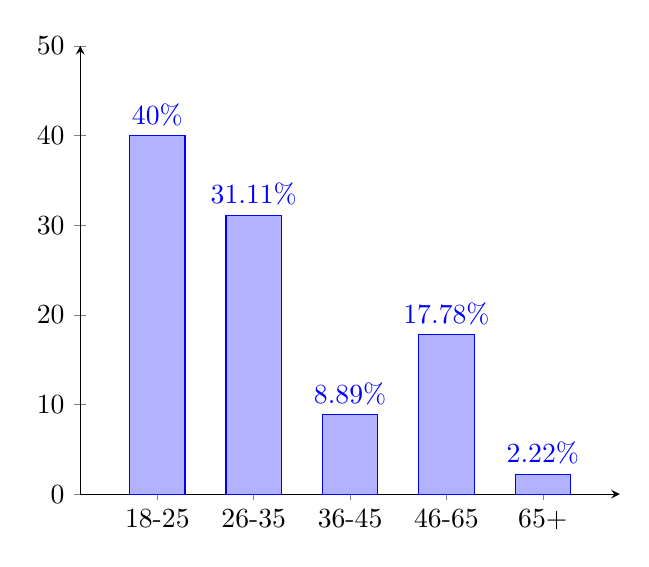
\begin{tikzpicture}
            \begin{axis}[
                ybar,
                bar width=20pt,
                ymin=0,
                ymax=50,
                symbolic x coords={18-25,26-35,36-45,46-65,65+},
                xtick=data,
                axis x line=bottom,
                axis y line=left,
                enlarge x limits=0.2,
                nodes near coords={\pgfmathprintnumber\pgfplotspointmeta\%}
            ]
                \addplot coordinates {(18-25,40) (26-35,31.11) (36-45,8.89) (46-65,17.78) (65+,2.22)};
            \end{axis}
        \end{tikzpicture}
        \caption{Participants by age group.}
        \label{fig:age}
    \end{center}
\end{figure}

$\bullet$ Genre

\begin{figure}[H]
    \begin{center}
        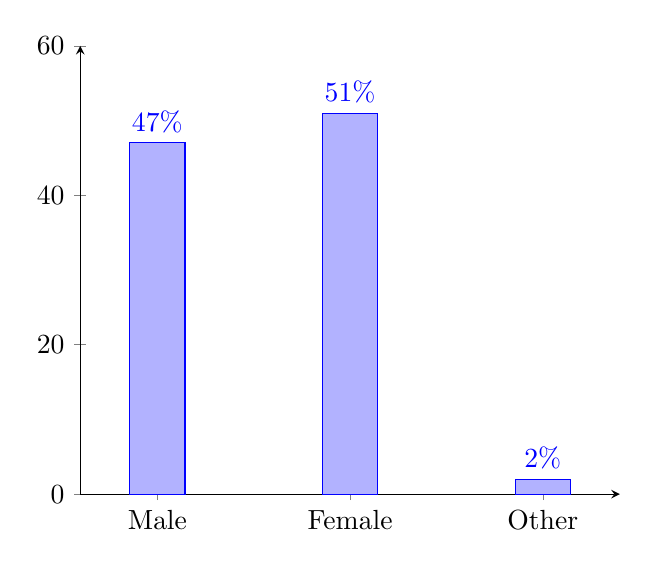
\begin{tikzpicture}
            \begin{axis}[
                ybar,
                bar width=20pt,
                ymin=0,
                ymax=60,
                symbolic x coords={Male,Female,Other},
                xtick=data,
                axis x line=bottom,
                axis y line=left,
                enlarge x limits=0.2,
                nodes near coords={\pgfmathprintnumber\pgfplotspointmeta\%}
            ]
                \addplot coordinates {(Male,47) (Female,51) (Other,2)};
            \end{axis}
        \end{tikzpicture}
        \caption{Participants by genre.}
        \label{fig:genre}
    \end{center}
\end{figure}

$\bullet$ Country

\begin{figure}[H]
    \begin{center}
        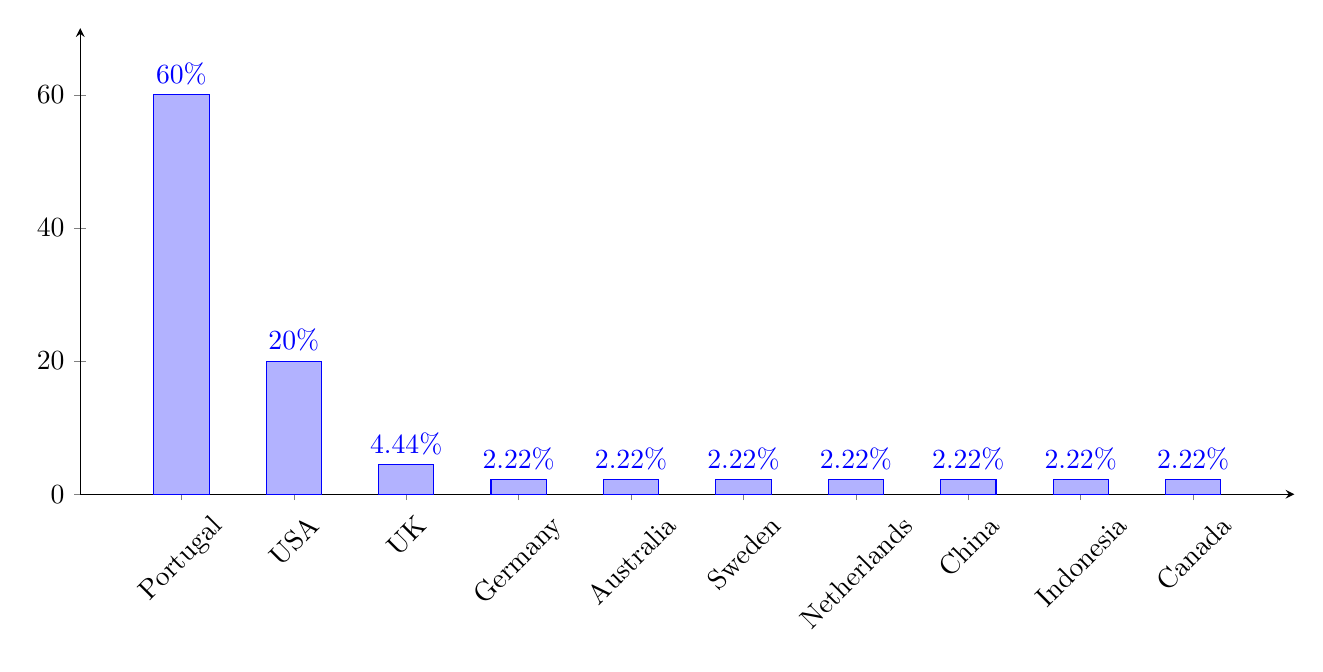
\begin{tikzpicture}
            \begin{axis}[
                height=7.5cm,
                width=17cm,
                ybar,
                bar width=20pt,
                ymin=0,
                ymax=70,
                symbolic x coords={Portugal,USA,UK,Germany,Australia,Sweden,Netherlands,China,Indonesia,Canada},
                xtick=data,
                xticklabel style={rotate=45},
                axis x line=bottom,
                axis y line=left,
                enlarge x limits=0.1,
                nodes near coords={\pgfmathprintnumber\pgfplotspointmeta\%}
            ]
                \addplot coordinates {(Portugal,60) (USA,20) (UK,4.44) (Germany,2.22) (Australia,2.22) (Sweden,2.22) (Netherlands,2.22) (China,2.22) (Indonesia,2.22) (Canada,2.22)};
            \end{axis}
        \end{tikzpicture}
        \caption{Participants by country.}
        \label{fig:country}
    \end{center}
\end{figure}

$\bullet$ District / State

$\bullet$ Level of Education

\begin{figure}[H]
    \begin{center}
        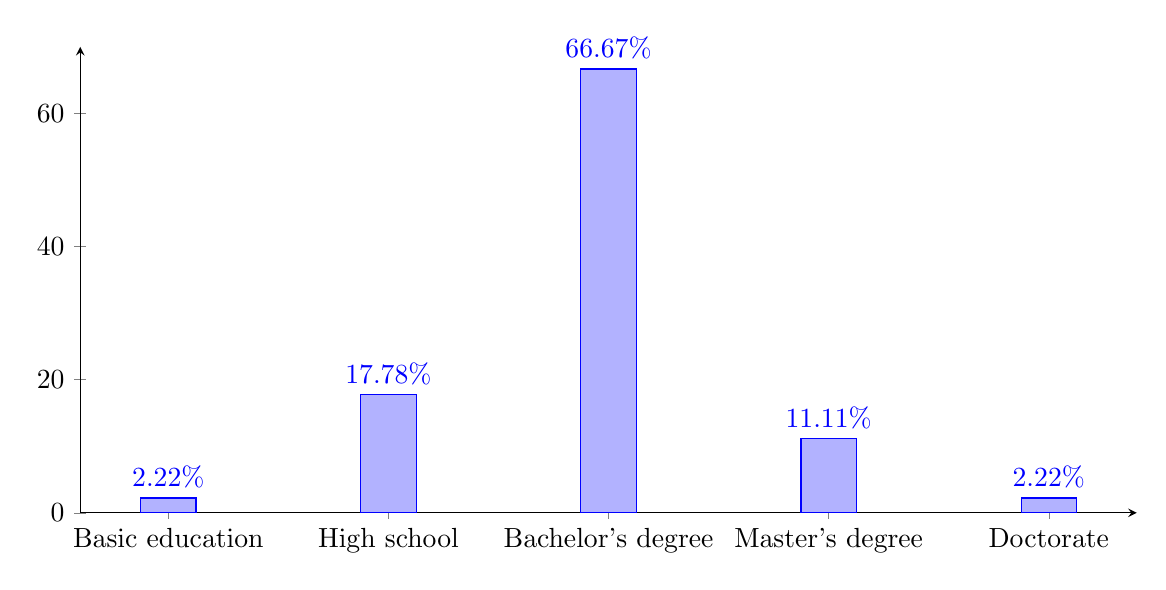
\begin{tikzpicture}
            \begin{axis}[
                height=7.5cm,
                width=15cm,
                ybar,
                bar width=20pt,
                ymin=0,
                ymax=70,
                symbolic x coords={Basic education,High school,Bachelor's degree,Master's degree,Doctorate},
                xtick=data,
                axis x line=bottom,
                axis y line=left,
                enlarge x limits=0.1,
                nodes near coords={\pgfmathprintnumber\pgfplotspointmeta\%}
            ]
                \addplot coordinates {(Basic education,2.22) (High school,17.78) (Bachelor's degree,66.67) (Master's degree,11.11) (Doctorate,2.22)};
            \end{axis}
        \end{tikzpicture}
        \caption{Participants by education level.}
        \label{fig:education}
    \end{center}
\end{figure}

$\bullet$ Professional area

$\bullet$ Annual income

\begin{figure}[H]
    \begin{center}
        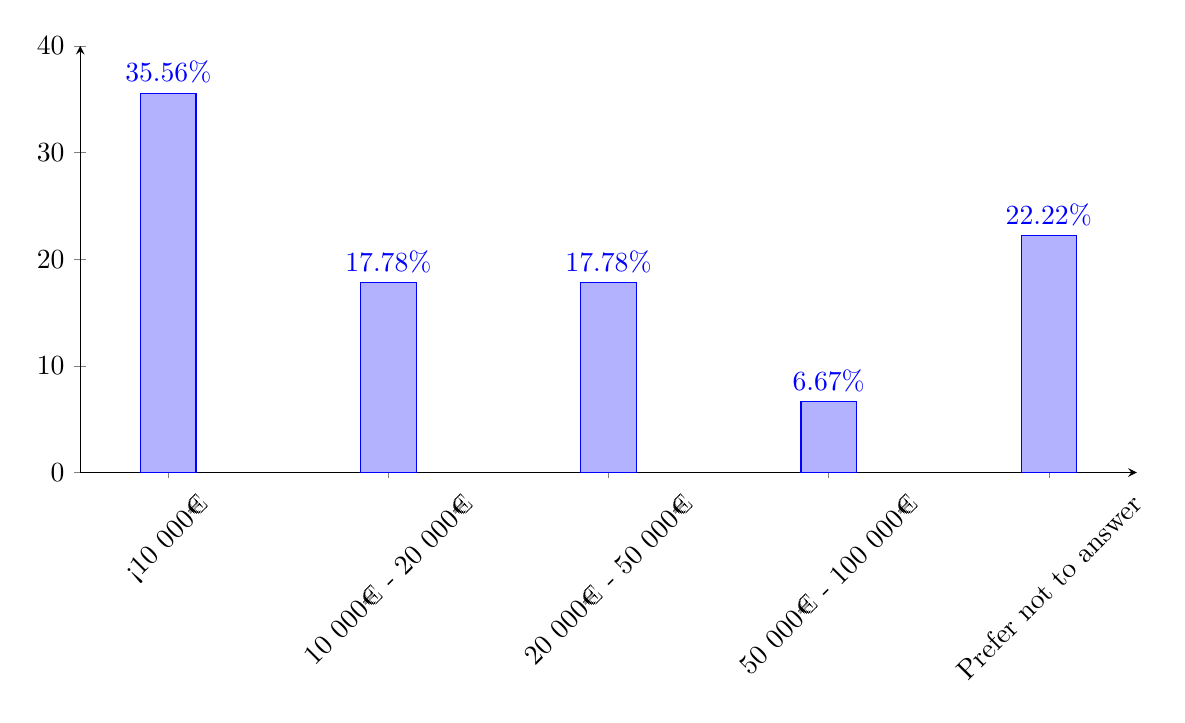
\begin{tikzpicture}
            \begin{axis}[
                height=7cm,
                width=15cm,
                ybar,
                bar width=20pt,
                ymin=0,
                ymax=40,
                symbolic x coords={<10 000€,10 000€ - 20 000€,20 000€ - 50 000€,50 000€ - 100 000€,Prefer not to answer},
                xtick=data,
                xticklabel style={rotate=45},
                axis x line=bottom,
                axis y line=left,
                enlarge x limits=0.1,
                nodes near coords={\pgfmathprintnumber\pgfplotspointmeta\%}
            ]
                \addplot coordinates {(<10 000€,35.56) (10 000€ - 20 000€,17.78) (20 000€ - 50 000€,17.78) (50 000€ - 100 000€,6.67) (Prefer not to answer,22.22)};
            \end{axis}
        \end{tikzpicture}
        \caption{Participants by annual income.}
        \label{fig:annual_income}
    \end{center}
\end{figure}

\clearpage

\section*{Appendix C: Usability Test}\label{appendix:usability_tests}

\subsection*{Tasks}

\begin{enumerate}
    \item Go to devices page \\
    \hspace*{0.46\textwidth}%
    \begin{tabularx}{0.2\textwidth}{@{}LR@{}}
        \textbf{\small Very difficult} & \textbf{\small Very easy}
    \end{tabularx}
    \begin{enumerate}
        \prop{Overall this task was?}
    \end{enumerate}
    \item Look up more information about one device
    \begin{enumerate}
        \prop{Overall this task was?}
    \end{enumerate}
    \item On the homepage look up more information about one device
    \begin{enumerate}
        \prop{Overall this task was?}
    \end{enumerate}
    \item Look up more information about this application
    \begin{enumerate}
        \prop{Overall this task was?}
    \end{enumerate}
    \item Create an account
    \begin{enumerate}
        \prop{Overall this task was?}
    \end{enumerate}
    \item Look up more information about privacy and Internet of Things on the app
    \begin{enumerate}
        \prop{Overall this task was?}
    \end{enumerate}
    \item Look up a tutorial on how to add a device
    \begin{enumerate}
        \prop{Overall this task was?}
    \end{enumerate}
    \item Add a device to the application
    \begin{enumerate}
        \prop{Overall this task was?}
    \end{enumerate}
    \item Update a device on the application
    \begin{enumerate}
        \prop{Overall this task was?}
    \end{enumerate}
\end{enumerate}

\subsection*{Usability Assessment}

\hspace*{0.47\textwidth}%
\begin{tabularx}{0.5\textwidth}{@{}LR@{}}
    \textbf{Strongly} & \textbf{Strongly} \\
    \textbf{Disagree} & \textbf{Agree} \\
\end{tabularx}

\begin{enumerate}
    \prop{I think that I would like to use this system frequently}

    \prop{I found the system unnecessarily complex}

    \prop{I thought the system was easy to use}

    \prop{I think that I would need the support of a technical person to be able to use this system}

    \prop{I found the various functions in this system were well integrated}

    \prop{I thought there was too much inconsistency in this system}

    \prop{I would imagine that most people would learn to use this system very quickly}

    \prop{I found the system very cumbersome to use}

    \prop{I felt very confident using the system}

    \prop{I needed to learn a lot of things before I could get going with this system}
\end{enumerate}

\clearpage

\section*{Appendix D: SUS}\label{appendix:sus}

Because a 7 point scale was used in the system usability scale, the scoring
differs slightly from the traditional 5 point scale. The following calculations were made:
for questions 1,3,5,7 and 9 the score is the participant marked scale position minus 1 and
for questions 2,4,6,8 and 10, the score is 7 minus the participant marked scale position;
then the sum of scores are multiplied by $5/3$ to obtain the overall value of the SUS.
Table \ref{table:sus_scoring} shows individual scores of participants and the average.

\begin{table}
    \centering
    \begin{tabular}{c c c c c c c c c c c c c}
        \hline
        \textbf{Participants} & \textbf{Q1} & \textbf{Q2} & \textbf{Q3} & \textbf{Q4} & \textbf{Q5} & \textbf{Q6} & \textbf{Q7} & \textbf{Q8} & \textbf{Q9} & \textbf{Q10} & \textbf{Corrected Sum} & \textbf{Score} \\
        \hline
        P1 & 7 & 1 & 7 & 1 & 7 & 1 & 7 & 6 & 7 & 1 & 55 & 91.67 \\
        \hline
        P2 & 7 & 2 & 6 & 1 & 7 & 1 & 7 & 1 & 7 & 1 & 58 & 96.67 \\
        \hline
        P3 & 6 & 1 & 4 & 1 & 7 & 1 & 7 & 1 & 5 & 2 & 54 & 90 \\
        \hline
        P4 & 6 & 1 & 7 & 1 & 7 & 1 & 7 & 1 & 7 & 1 & 59 & 98.33 \\
        \hline
        P5 & 5 & 1 & 7 & 6 & 7 & 1 & 7 & 1 & 7 & 2 & 51 & 85 \\
        \hline
        P6 & 6 & 1 & 7 & 1 & 7 & 1 & 7 & 1 & 7 & 2 & 58 & 96.67 \\
        \hline
        P7 & 6 & 2 & 6 & 7 & 7 & 2 & 7 & 2 & 6 & 2 & 47 & 78.33 \\
        \hline
        \textbf{Average} & 6.14 & 1.29 & 6.29 & 2.57 & 7 & 1.14 & 7 & 1.86 & 6.71 & 1.57 & 54.57 & 90.95 \\
        \hline
    \end{tabular}
    \vspace{1em}
    \caption{SUS scores of participants.}
    \label{table:sus_scoring}
\end{table}
